\documentclass[aps,prapplied,reprint,superscriptaddress,longbibliography]{revtex4-2}
\usepackage[T1]{fontenc}
\usepackage[utf8]{inputenc}
\usepackage{amsmath,amssymb,bm,graphicx,booktabs}
\usepackage{xcolor}
\usepackage{microtype}
\usepackage[hidelinks]{hyperref}

\newcommand{\vct}[1]{\boldsymbol{#1}}
\newcommand{\Eloc}{E_{\mathrm{loc}}}
\newcommand{\DTV}{D_{\mathrm{TV}}}
\newcommand{\DKL}{D_{\mathrm{KL}}}
\newcommand{\avg}[1]{\left\langle #1\right\rangle}
\newcommand{\betaeff}{\beta_{\mathrm{eff}}}
\newcommand{\betahw}{\beta_{\mathrm{hw}}}
\newcommand{\panel}[2]{\begin{minipage}[t]{#1\textwidth}\centering #2\end{minipage}}

% ---------------------------------------------------------------------------
% \missing{}: visually flags analyses/figures/code that do not exist yet.
% Every use is also logged in MISSING.md at the repository root of this draft.
% ---------------------------------------------------------------------------
\newcommand{\missing}[1]{%
  \begin{quote}\color{red!70!black}\itshape
  [MISSING ANALYSIS -- #1]
  \end{quote}%
}
\newcommand{\missinginline}[1]{\textcolor{red!70!black}{\itshape[missing: #1]}}

\begin{document}

\title{Pooled Conditional Thermometry for Quantum-Annealer-Assisted\\ Neural Quantum States}

\author{Philipp Hanussek}
\email{philipp.hanussek@etu.sorbonne-universite.fr}
\affiliation{Institute of Theoretical and Applied Informatics, Polish Academy of Sciences, Ba\l{}tycka 5, Gliwice, 44-100, Poland}
\affiliation{Sorbonne Universit\'e, Facult\'e des Sciences et Ing\'enierie, 75005 Paris, France}

\author{Zakaria Mzaouali}
\email{z.mzaouali@extern.fz-juelich.de}
\affiliation{J\"ulich Supercomputing Centre, Forschungszentrum J\"ulich, Wilhelm-Johnen-Stra{\ss}e, J\"ulich, 52428, Germany}
\affiliation{Institut f\"ur Theoretische Physik, Universit\"at T\"ubingen, Auf der Morgenstelle 14, 72076 T\"ubingen, Germany}

\author{\L{}ukasz Pawela}
\affiliation{Institute of Theoretical and Applied Informatics, Polish Academy of Sciences, Ba\l{}tycka 5, Gliwice, 44-100, Poland}
\affiliation{Quantumz.io Sp.\ z o.\ o., Pu\l{}awska 12/3, 02-566 Warsaw, Poland}

\author{Bart\l{}omiej Gardas}
\email{bgardas@iitis.pl}
\affiliation{Institute of Theoretical and Applied Informatics, Polish Academy of Sciences, Ba\l{}tycka 5, Gliwice, 44-100, Poland}
\affiliation{Quantumz.io Sp.\ z o.\ o., Pu\l{}awska 12/3, 02-566 Warsaw, Poland}

\date{\today}

\begin{abstract}
Quantum annealers can supply configurations for neural-network variational Monte Carlo, but a returned sample is only useful if its distribution -- not merely its energy -- is known. We introduce a partition-function-free, online conditional-thermometry estimator for restricted-Boltzmann-machine (RBM) wavefunctions sampled by a quantum annealer: every visible configuration observed during training is treated as its own conditioning vector, and all paired hidden observations are pooled into a single effective-inverse-temperature estimate, at no additional device cost. We derive this estimator as a conditional maximum-likelihood problem, relate it to the least-squares construction used in earlier work, and quantify its residual disagreement with the full visible distribution on small transverse-field-Ising-model (TFIM) systems where exact enumeration is possible. Building on this diagnostic, we benchmark two generations of D-Wave hardware (Pegasus, Zephyr) against classical Markov-chain samplers and a field-programmable-gate-array (FPGA) sampler under an independently validated time-to-accuracy criterion, and we report the hardware-resource cost (physical qubits, chain length, embedding success) of the quantum-annealer arm alongside its device time. \missinginline{headline result pending re-run of items in Sec.~\ref{sec:limitations}} We find [PLACEHOLDER: state the corrected, size- and criterion-conditional crossover result once independently validated TTA data are available] rather than an unconditional claim that quantum annealing overtakes classical sampling.
\end{abstract}

\maketitle

\section{Introduction}
\label{sec:intro}

Variational Monte Carlo (VMC) approximates a quantum ground state by optimizing a parametrized trial wavefunction against expectation values estimated from sampled configurations. Restricted Boltzmann machines (RBMs) are an attractive choice of trial state because their amplitudes and logarithmic derivatives factorize over a hidden layer and can be evaluated in closed form~\cite{Carleo2017,Sorella2001}. Their practical accuracy, however, depends on three largely independent things: whether the sampler used during training actually draws from the state's Born distribution, whether the network's connectivity and sign structure can represent the target state at all, and whether the reported convergence is confirmed by an evaluation that does not share the training sampler's own biases.

A quantum annealer can supply the configurations used in this loop: a programmable Ising energy is realized on the device, and repeated anneals return classical spin strings~\cite{Gardas2018}. Whether those strings behave like Gibbs samples at some effective temperature is an empirical question, not a guarantee of the hardware. Benedetti \textit{et al.} showed that this effective temperature is instance dependent~\cite{Benedetti2016}; Nelson \textit{et al.} examined the conditions under which annealer output resembles thermal sampling at all~\cite{Nelson2022}. Any procedure that uses annealer samples inside an RBM training loop therefore needs an online, per-instance estimate of that effective temperature, obtained without extra hardware calls and without assuming the partition function is tractable.

Two recent papers make this a crowded claim on their own terms, and the present contribution must be stated more narrowly than ``online calibration from training samples'' as a result. Goto and Ohzeki already reuse visible and hidden samples generated during RBM training to calibrate more than one internal annealer parameter online, benchmarking directly against Gibbs sampling and contrastive divergence~\cite{Goto2025}. Kim, Gyhm, and Park go further and report that a diabatic-annealing sampler, corrected by an analytical temperature-rescaling method, gives RBM training with faster convergence and lower validation error than classical sampling outright~\cite{Kim2026}. What we isolate below is not ``online, sample-reusing calibration'' in general -- both of the above already do that -- but the specific \emph{pooled, no-requery} construction of Sec.~\ref{sec:cem-ls} and a deliberately narrower empirical claim: Sec.~\ref{sec:limitations} reports one criterion-specific, statistically marginal ordering rather than the general classical-vs-quantum superiority Kim \textit{et al.} assert.

\subsection{Pooled conditional thermometry: the central contribution}

Kubo and Goto introduced conditional expectation matching (CEM): the hidden-unit conditional means of an RBM, $\mathbb E[h_j\mid v]=\tanh(\beta\phi_j(v))$, are fit to the corresponding sampled hidden bits at a \emph{fixed} visible configuration, giving a partition-function-free estimate of $\beta$~\cite{Kubo2025,Kubo2026}. The contribution we isolate and develop here is the \emph{pooled} version of this idea: rather than querying the sampler again at a fixed $v$, every visible configuration $v^{(r)}$ produced during ordinary training is treated as its own conditioning vector, and all $(v^{(r)},h^{(r)})$ pairs already generated by stochastic reconfiguration (SR) are pooled into one least-squares (Sec.~\ref{sec:cem-ls}) estimate of a single effective inverse temperature $\betaeff$. This requires no additional annealer queries and no evaluation of $Z_\theta$.

We are explicit about what this estimator does and does not certify. A perfect fit of the hidden conditional means at a given $\beta$ is compatible with an arbitrarily wrong visible marginal (Sec.~\ref{sec:cem-limits}); consequently, a pooled-CEM estimate is a diagnostic of the hidden-layer response scale, not a certificate that the sampler reproduces $\pi_\theta(v)=|\psi_\theta(v)|^2$. Separating these two claims -- and building an independent-evaluation pipeline that tests the second one directly -- is the paper's second contribution.

\subsection{Related constraints: representation and validation}

Two further limitations are independent of thermometry and are treated as such rather than folded into a single ``competitiveness'' narrative. First, connectivity: a dense RBM does not fit natively on an annealer's coupler graph, so either minor embedding or an explicitly sparse, hardware-native mask must be used, and the two have different accuracy-vs-resource trade-offs~\cite{LeRoux2008}. Second, sign structure: a positive-amplitude RBM can only represent target states whose off-diagonal Hamiltonian matrix elements are non-positive in the computational basis~\cite{Bravyi2008}; the Marshall transformation supplies this sign for a bipartite nearest-neighbor antiferromagnet~\cite{Marshall1955} but not for a frustrated one~\cite{Richter1994,Voigt2000}. Neither limitation is repaired by a better sampler, and neither is the subject of this paper's central claim; we report both only insofar as they interact with the resource accounting in Sec.~\ref{sec:resources}.

\subsection{Enumerated contributions}

\begin{enumerate}
\item A pooled conditional-thermometry estimator for annealer-sampled RBMs, built on the least-squares objective of prior work (Sec.~\ref{sec:thermometry}), together with an explicit statement of what agreement of hidden conditional means does and does not imply about the visible distribution (Sec.~\ref{sec:cem-limits}).
\item An independent validation protocol -- exact enumeration at small $N$, long independent reference sampling at larger $N$, with training and evaluation using disjoint random streams -- applied to frozen, checkpointed ansätze, so that a reported convergence is confirmed by an estimator that does not share the training sampler's bias (Sec.~\ref{sec:validation}).
\item A quantitative account of the residual gap between the fitted effective temperature and the true visible distribution, on transverse-field-Ising systems small enough for exact enumeration (Sec.~\ref{sec:calibration}).
\item Independently validated time-to-accuracy curves across a grid of convergence tolerances $\epsilon$ and fields $h$, replacing a single-threshold, single-field time-to-$\epsilon$ statistic with its criterion dependence made explicit (Sec.~\ref{sec:tta}).
\item A joint accounting of device time, end-to-end wall time, and quantum-annealer hardware resources (physical qubits, chain length, chain-break fraction, embedding success rate) used to reach that accuracy, so that a timing comparison is read together with the resources it consumed (Sec.~\ref{sec:resources}).
\item An explicit statement of the conditions under which a quantum-annealer/FPGA crossover is observed, replacing an unconditional claim with the size-, field-, and tolerance-dependent statement the data actually support (Sec.~\ref{sec:limitations}).
\end{enumerate}

This paper is deliberately narrower than the research-stay report it is drawn from. Sparse hardware-native RBMs, parallel embeddings, and the Marshall-sign study are retained only as short, explicitly scoped appendices (App.~\ref{app:sparse}--\ref{app:marshall}); they support the resource-accounting discussion but are not part of the central thermometry-and-validation claim.

\section{Pooled conditional thermometry}
\label{sec:thermometry}

\subsection{RBM wavefunction and sampling model}
\label{sec:setup}

We use Pauli operators $\sigma_i^\mu$, $\mu\in\{x,y,z\}$, and computational-basis configurations $v=(v_1,\dots,v_N)$, $v_i=\pm1$. The transverse-field Ising chain,
\begin{equation}
H_{\mathrm I}=-J\sum_{i=1}^N\sigma_i^z\sigma_{i+1}^z-\Gamma\sum_{i=1}^N\sigma_i^x,
\label{eq:ising}
\end{equation}
with $J=1$ and periodic boundaries, supplies an exactly solvable reference energy for even $N$~\cite{Lieb1961,He2017} against which the validation procedure of Sec.~\ref{sec:validation} is checked.

An RBM with $N$ visible spins $v$, $M$ hidden spins $h$, biases $(a,b)$, and couplings $W$ defines the auxiliary energy $\mathcal E_\theta(v,h)=\sum_i a_iv_i-\sum_jb_jh_j-\sum_{ij}W_{ij}v_ih_j$. Writing $\phi_j(v)=b_j+\sum_iW_{ij}v_i$, the marginal amplitude, Born distribution, and hidden conditional means are
\begin{align}
A_\theta(v)&=e^{-\frac12\sum_ia_iv_i}\prod_{j=1}^M[2\cosh\phi_j(v)]^{1/2},\label{eq:amplitude}\\
\pi_\theta(v)&=A_\theta(v)^2/Z_\theta,\qquad \psi_\theta(v)=s(v)\sqrt{\pi_\theta(v)},\label{eq:born}\\
\mathbb E[h_j\mid v]&=\tanh\phi_j(v).\label{eq:condmean}
\end{align}
The sign $s(v)$ is fixed (Sec.~\ref{sec:intro}); it plays no role in this section. Parameters are updated with stochastic reconfiguration (SR) using the local energy $\Eloc(v)$ and the logarithmic derivatives of $A_\theta$~\cite{Sorella1998,Sorella2001}, exactly as in prior work on this system; we do not modify the optimizer and record it here only to fix notation for Sec.~\ref{sec:resources}.

A quantum annealer used as a sampler returns joint configurations $(v^{(r)},h^{(r)})_{r=1}^S$ at each SR iteration. If these were exact samples from the Gibbs distribution $q(v,h)\propto e^{-\betahw\mathcal E_\theta(v,h)}$ at some device inverse temperature $\betahw$, rescaling the submitted coefficients by $1/\beta_x$ would give an effective inverse temperature $\betaeff=\betahw/\beta_x$, and the corresponding visible marginal would be
\begin{equation}
\pi_{\theta,\beta}(v)=\frac{e^{-\beta a\cdot v}\prod_j2\cosh[\beta\phi_j(v)]}{Z_{\theta,\beta}}.
\label{eq:tempered}
\end{equation}
Equation~\eqref{eq:tempered} is a model to be tested against the sampler's actual output, not an identity that quantum annealing satisfies by construction.

\subsection{Least-squares pooled CEM}
\label{sec:cem-ls}

The pooled least-squares estimator reuses the $(v^{(r)},h^{(r)})$ pairs already produced by SR -- no fixed-condition re-query of the device is needed -- and fits
\begin{equation}
\widehat\beta_{\mathrm{LS}}=\operatorname*{arg\,min}_{\beta>0}\;
\mathcal L(\beta)=\sum_{r=1}^S\sum_{j=1}^M\big[h_j^{(r)}-\tanh(\beta\phi_j(v^{(r)}))\big]^2,
\label{eq:cem-ls}
\end{equation}
minimized by bounded scalar search over $\beta\in[0.01,50]$ in the implementation we audit. This is the estimator used in the source report and is the one for which Sec.~\ref{sec:calibration} reports residual visible-distribution error.

\subsection{What agreement of hidden conditionals does not imply}
\label{sec:cem-limits}

Write $m_j(v)=\mathbb E_q[h_j\mid v]$ for the sampler's true hidden conditional mean. The expected per-configuration loss of Eq.~\eqref{eq:cem-ls} decomposes as
\begin{equation}
\frac{\mathbb E_q[\mathcal L(\beta)]}{S}=\sum_j\mathbb E_{q(v)}\Big[\operatorname{Var}_q(h_j\mid v)+[m_j(v)-\tanh(\beta\phi_j(v))]^2\Big].
\label{eq:conditionalproof}
\end{equation}
If the hidden conditionals are exactly correct at some $\beta_0$, that value minimizes Eq.~\eqref{eq:conditionalproof} \emph{regardless of the visible marginal $q(v)$}. A minimal counterexample makes this concrete: one visible and one hidden spin, $a=0$, $b=0.2$, $W=0.4$, target $\beta=1$, so the two conditional fields are $\mp0.2,\allowbreak 0.6$ depending on $v=\mp1$. A sampler that places all visible weight on $v=-1$ but draws $h$ from the correct conditional at that $v$ reproduces $\widehat\beta_{\mathrm{LS}}=1$ exactly, while its visible total-variation error is
\begin{equation}
\DTV(q(v),\pi_\theta(v))=\frac{\cosh(0.6)}{\cosh(-0.2)+\cosh(0.6)}\approx0.5375.
\label{eq:counterexample}
\end{equation}
Any pooled-CEM estimate is therefore a diagnostic of the hidden-layer response scale, not a certificate of the full visible distribution; Sec.~\ref{sec:calibration} reports the residual visible-distribution error directly rather than inferring it from $\widehat\beta$ alone.

\section{Independent validation methodology}
\label{sec:validation}

The central methodological weakness identified in review of the source report is that ``convergence'' was determined from the rolling mean of the \emph{training-time} logged energy (Eqs.~\eqref{eq:rollingmean}--\eqref{eq:crossing} below), computed from samples drawn by the very sampler under test. The local energy is an unbiased estimator of the variational energy $E_\theta=\sum_v\pi_\theta(v)\Eloc(v)$ only when its samples are drawn from $\pi_\theta$ itself (Eq.~\eqref{eq:born}); if a sampler returns a distorted distribution $q\ne\pi_\theta$, it can simultaneously bias the SR update, bias its own logged training energy, and produce an apparently early threshold crossing, all consistently with one another. Because the pooled-CEM diagnostic of Sec.~\ref{sec:thermometry} does not certify the visible distribution (Sec.~\ref{sec:cem-limits}), a QPU-trained ansatz's convergence cannot be taken at face value from its own training log. This section specifies the independent evaluator that Secs.~\ref{sec:calibration}--\ref{sec:tta} then apply.

\subsection{Frozen-ansatz re-evaluation protocol}
\label{sec:protocol}

At each checkpointed SR iteration $t$, the parameters $\theta_t$ are frozen and evaluated by a procedure that shares no randomness with the training sampler:
\begin{enumerate}
\item \textbf{Exact enumeration, $N\lesssim20$--$24$.} $E_{\theta_t}=\sum_v\pi_{\theta_t}(v)\Eloc(v)$ is computed by direct summation over all $2^N$ configurations, giving a training-independent, sampling-noise-free reference energy and, via $\pi_{\theta_t}$, an exact visible-distribution reference against which any sampler's histogram can be compared with $\DTV$ or $\DKL$.
\item \textbf{Independent multi-chain reference sampling, larger $N$.} A long block-Gibbs or Metropolis chain (Eq.~\eqref{eq:condmean}), seeded independently of the training run and of any QPU calls, estimates $\widetilde E_q=\sum_vq(v)\Eloc(v)$ with multiple independent chains, reported mixing diagnostics (e.g.\ split-$\hat R$ or an integrated autocorrelation time), and confidence intervals corrected for the resulting autocorrelation rather than treated as i.i.d.
\item \textbf{Energy variance as a second criterion.} Because an exact eigenstate has $\operatorname{Var}_{\pi_\theta}(\Eloc)=0$, a checkpoint is reported with both its estimated energy error and its estimated local-energy variance; a small variance under correct averaging is evidence of proximity to \emph{an} eigenstate, not by itself evidence that it is the ground state.
\end{enumerate}
A crossing at tolerance $\epsilon$ (Sec.~\ref{sec:tta}) is declared only when an upper confidence bound on the \emph{independently} estimated energy error, from step 1 or 2, falls below $\epsilon$. Until this evaluation is performed, we follow the evaluation's suggested terminology and refer to the training-log-based statistic used in the source report as a seed \emph{satisfying the training-energy criterion}, not as a validated seed.

\subsection{Training-time crossing statistic, for reference}
\label{sec:trainingcrossing}

The source report's crossing statistic, which the re-evaluation above supersedes, uses a rolling mean of the logged training energy $\widehat E_t$ over a window $w$,
\begin{equation}
\overline E_t=\frac1{t-t_0+1}\sum_{\tau=t_0}^t\widehat E_\tau,\quad t_0=\max(1,t-w+1),\quad \delta_t=\frac{|\overline E_t-E_0|}{N},
\label{eq:rollingmean}
\end{equation}
and the first sustained crossing $t^\star=\min\{t\le T-w+1:\delta_s<\epsilon\ \forall s\in\{t,\dots,t+w-1\}\}$, undefined within budget $T$ if no such $t^\star$ exists. We retain this definition because Sec.~\ref{sec:tta} reports both the training-time and the independently validated crossing side by side, so that the size of the gap between them -- rather than only the corrected number -- is visible.

\missing{\textbf{Implementation and execution of the frozen-ansatz re-evaluator.} No script in the audited repository re-evaluates a checkpointed RBM by exact enumeration or by an independent, separately seeded sampling chain; the only enumeration code found operates on small hand-built diagnostic examples (Sec.~\ref{sec:cem-limits}), not on checkpoints saved from a training run (Sec.~\ref{sec:code-gaps}, item T2). This is, in the evaluation's words, ``the most important methodological repair'' and is listed first among the placeholders in Sec.~\ref{sec:code-gaps} because every downstream number in Secs.~\ref{sec:calibration}--\ref{sec:tta} that is labelled ``independently validated'' depends on it. Concretely still needed: (i) a checkpoint-loading harness that reconstructs $\theta_t$ without touching the training RNG state; (ii) an exact-enumeration evaluator for $N\le24$; (iii) an independent multi-chain Gibbs/Metropolis evaluator with a mixing diagnostic for larger $N$; (iv) re-running both over the archived checkpoints for at least the cells entering Fig.~\ref{fig:tta-grid} [PLACEHOLDER] and Table~\ref{tab:crossover} [PLACEHOLDER].}

\section{Calibration accuracy and residual non-Gibbs distortion}
\label{sec:calibration}

This section reports what is already measurable with exact enumeration at small $N$: how far a calibrated annealer sample actually sits from the intended visible distribution, independent of any $\betaeff$ fit.

\subsection{Effect of input scale and automatic normalization}

Figure~\ref{fig:autoscale} sweeps the input coefficient scale $\beta_x$ on a small ($N=8$) Pegasus-embedded network. With the solver's automatic coefficient normalization enabled, rescaling all programmed coefficients by $1/\beta_x$ has little effect on either $\DTV(\widehat q,\pi_\theta)$ or the fitted $\widehat\beta_{\mathrm{LS}}$: normalization divides by a quantity that scales with the same factor, canceling the intended change. With normalization disabled, both quantities respond to $\beta_x$: the recorded $\DTV$ falls from $\approx0.63$ to $\approx0.30$ near $\beta_x=5$ before rising again, against a finite-sample reference of $\approx0.19$ at this sample count. Reaching the right scale improves the histogram; it does not make the sampled distribution statistically indistinguishable from an ideal sample of $\pi_\theta$ at that sample count.

\begin{figure}[t]
\centering
\panel{.48}{\textbf{(a)}\\
\includegraphics[width=\linewidth]{figures/dtv_autoscale_dtv_N8.pdf}}\hfill
\panel{.48}{\textbf{(b)}\\
\includegraphics[width=\linewidth]{figures/dtv_autoscale_beta_N8.pdf}}
\caption{Effect of automatic coefficient normalization on a small ($N=8$) Pegasus-embedded network. (a) Total-variation distance to the enumerated $\pi_\theta$. (b) Fitted $\widehat\beta_{\mathrm{LS}}$ (Eq.~\eqref{eq:cem-ls}). Disabling normalization lets the input scale $\beta_x$ change the sampled law; enabling it cancels the attempted adjustment. The reference line is a finite-sample floor at this sample count, not a lower bound.}
\label{fig:autoscale}
\end{figure}

\subsection{Sampler comparison against the exact trial distribution}

Figure~\ref{fig:classical} compares classical samplers against the exactly enumerated distribution of trained $N=M=8$ networks at two field values. Metropolis and block Gibbs sampling remain close to the finite-sample reference across the tested effort range; simulated annealing starts far from it at low effort and approaches the other two as its schedule lengthens. A separate audit of the source report (\texttt{audyt\_cld\_bg.md}, finding O2: ``No matched QPU-versus-classical sampling-quality benchmark'') asked for exactly this comparison on a QPU. We obtained one directly: 10 fresh Pegasus draws (200 reads each, live \texttt{Advantage\_system6}, $\beta_x=2.0$) on a small trained network ($N=8$, from the surviving \texttt{cem\_validation} checkpoint), scored against the same exact-enumeration reference used throughout this section -- $\DTV(\widehat q,\pi_\theta)=0.637$ (IQR $[0.620,0.641]$) and $\widehat\beta_{\mathrm{LS}}=1.80$ (IQR $[1.66,1.85]$) across the 10 seeds. This sits well above the classical samplers' finite-sample floor in Fig.~\ref{fig:classical} -- a real, live-hardware instance of the residual non-Gibbs distortion this section is built around, not merely the single differently-scoped auto-scale point of Fig.~\ref{fig:autoscale}.

\begin{figure}[t]
\centering
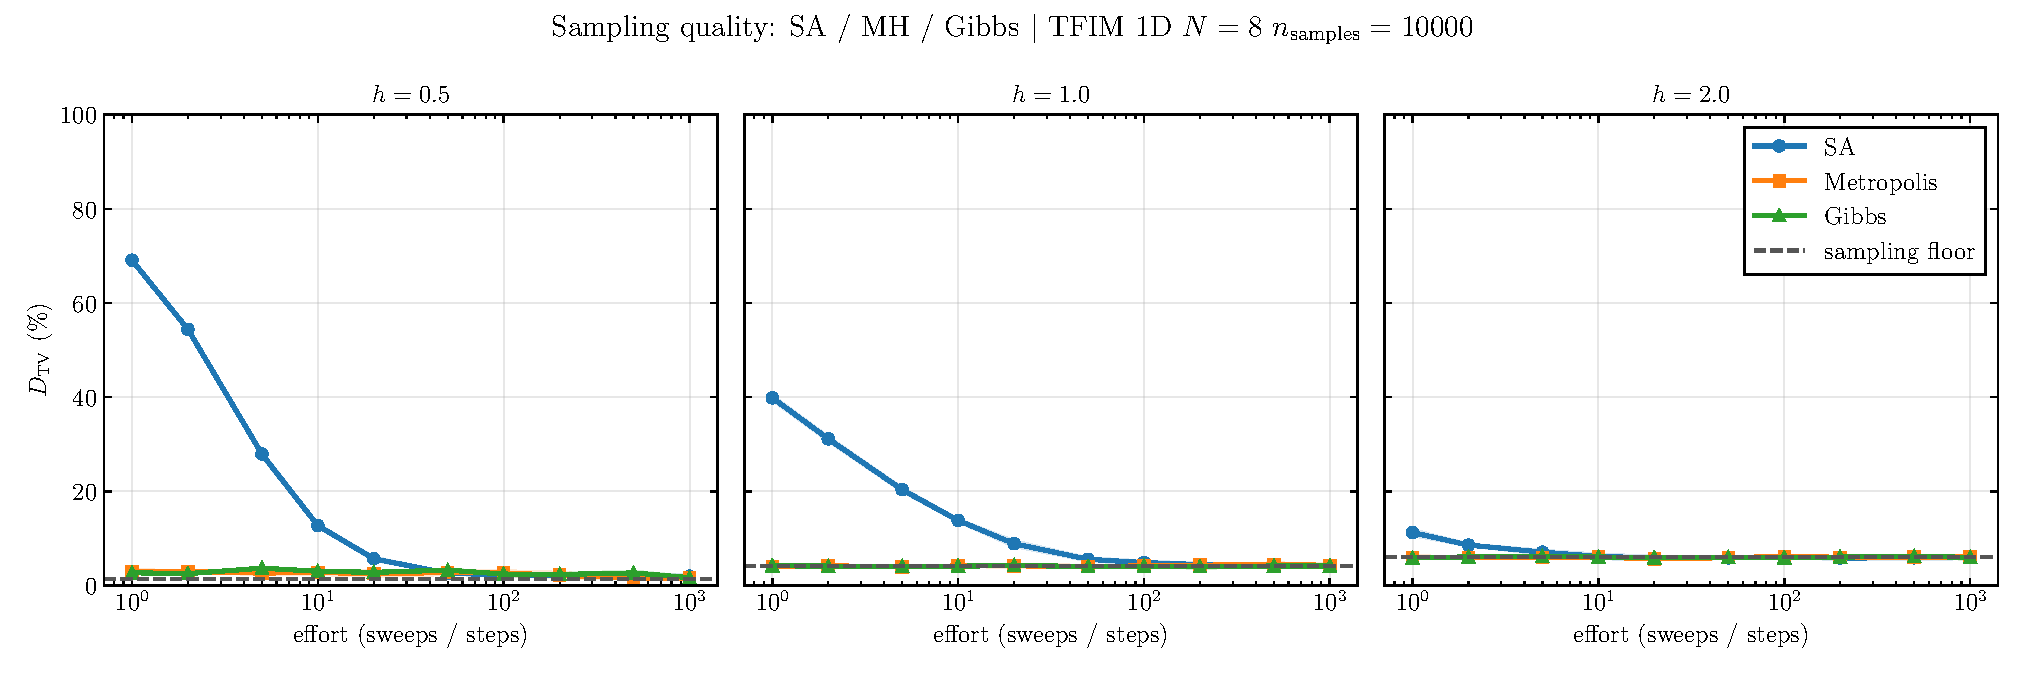
\includegraphics[width=\linewidth]{figures/dtv_classical_N8_M8.pdf}\\[2pt]
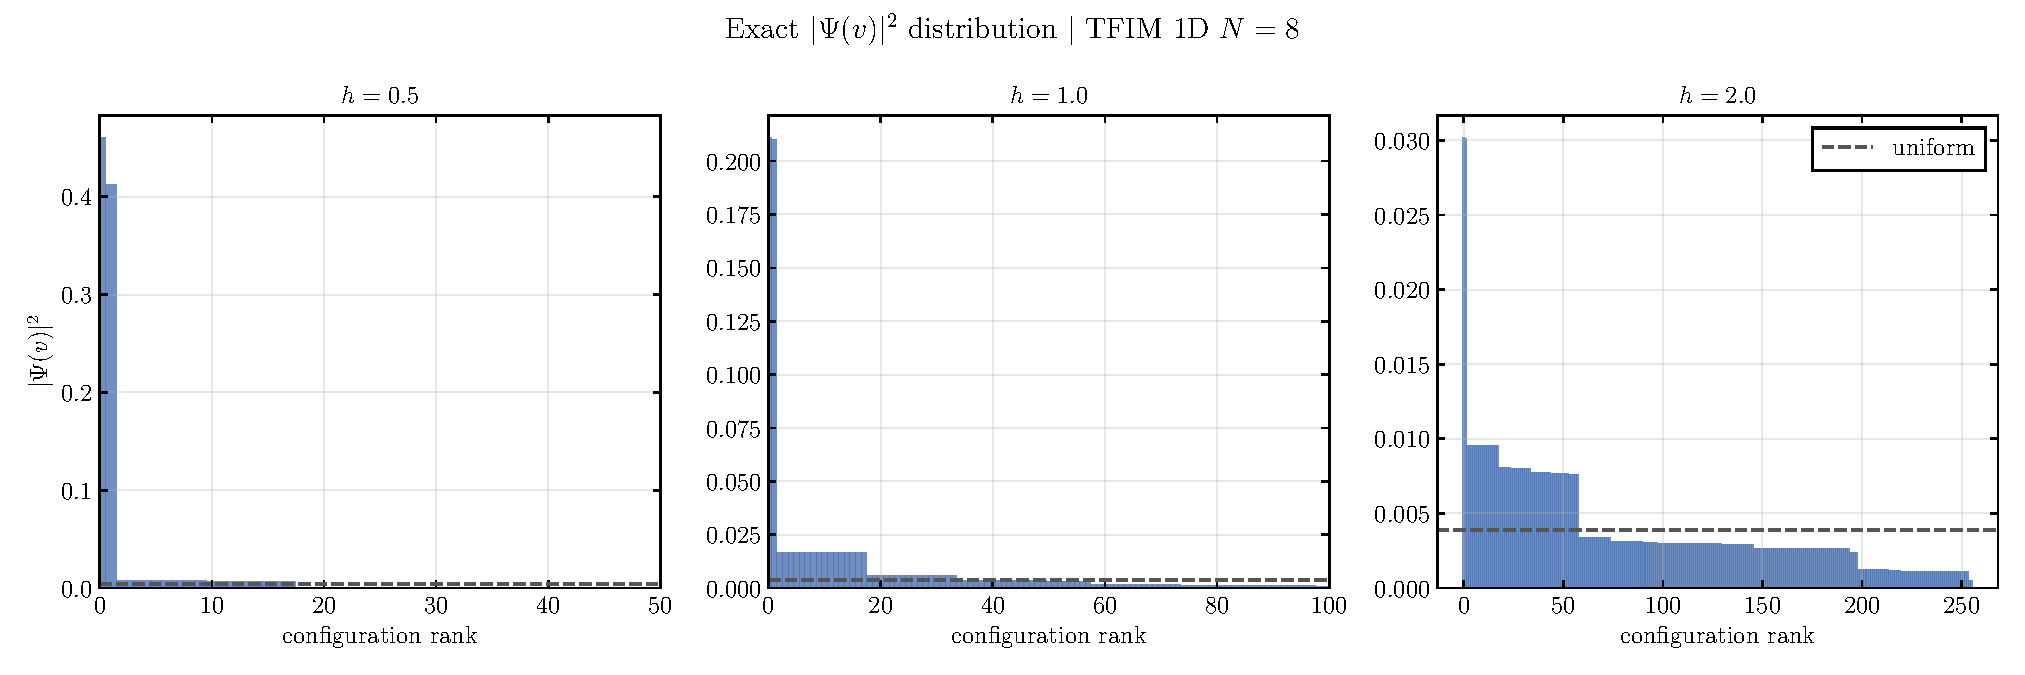
\includegraphics[width=\linewidth]{figures/dtv_classical_N8_M8_dist.pdf}
\caption{Sampling diagnostics for trained $N=M=8$ Ising networks at $h=0.5$ and $h=2$. Top: total-variation distance from the enumerated trial distribution vs.\ sampling effort. Bottom: ranked probabilities of the trial distribution itself.}
\label{fig:classical}
\end{figure}

A matched comparison turns out to already exist in the archived training logs, just never plotted this way. Every training run at $N\le16$ logs \texttt{kl\_exact}: the exact-enumeration $\DKL(\widehat q\Vert\pi_\theta)$ between that iteration's empirical sample histogram and the \emph{current} $\theta$'s own exactly enumerated Born distribution (\texttt{src/encoder.py}, gated by \texttt{KL\_EXACT\_MAX\_N=16}), computed identically for classical and QPU-driven runs. Figure~\ref{fig:kl-solver} plots it against SR iteration for all six solvers at $N=8,16$, closing audit finding O2 above with no new experiments.

\paragraph{Status.} \textbf{O2: closed}, in substance: a matched classical-vs-QPU sampling-quality comparison, on identical axes, now exists at $N=8,16$. One narrower part of the original finding is not fully addressed -- it also asked for the fitted $\beta_{\mathrm{eff}}$ to be reported alongside; we show CEM's downstream effect on distributional fidelity (Fig.~\ref{fig:kl-cem}) rather than tabulating $\widehat\beta_{\mathrm{LS}}$ itself next to Fig.~\ref{fig:kl-solver}.

\begin{figure*}[t]
\centering
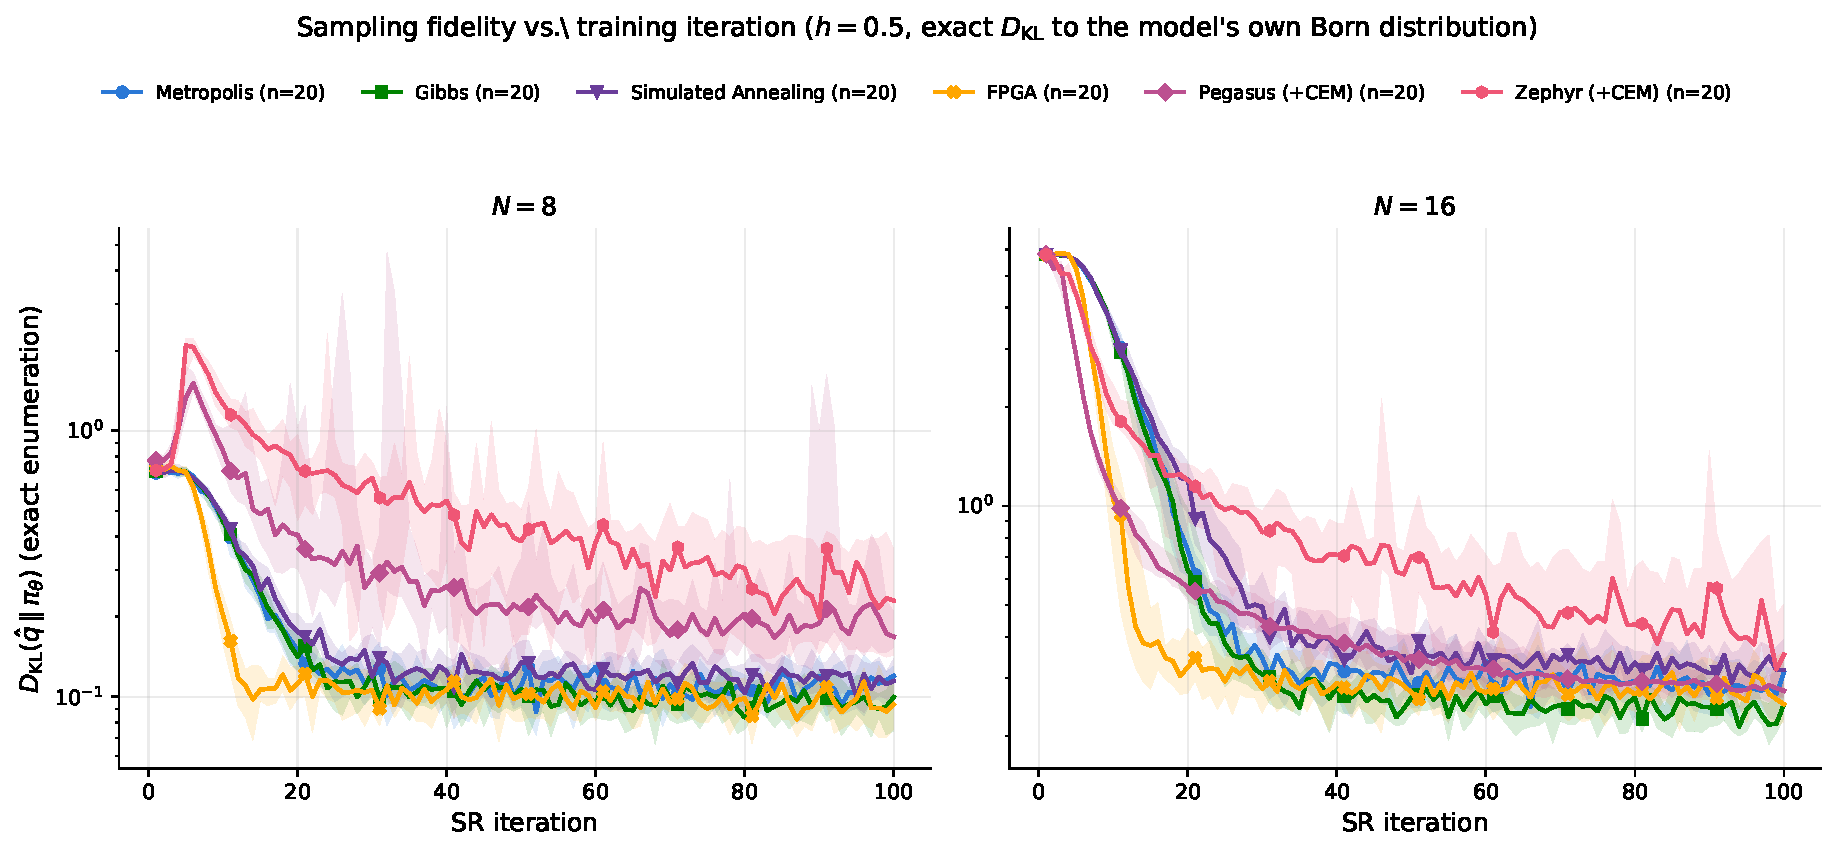
\includegraphics[width=\textwidth]{figures/reanalysis/fig_kl_exact_solver_comparison.pdf}
\caption{Exact $\DKL(\widehat q\Vert\pi_\theta)$ vs.\ SR iteration, $h=0.5$, $N=8,16$ (median and IQR band, 20 seeds per solver). Classical MCMC (Metropolis, Gibbs, simulated annealing) and FPGA converge to a common, tight floor by iteration $\sim\!20$--$30$. Pegasus(+CEM) and Zephyr(+CEM) settle above that floor, with visibly wider bands -- a directly quantified, exact-enumeration version of the ``residual non-Gibbs distortion'' this section otherwise only measures indirectly through $\DTV$ at one instance. All curves start high and decline: the RBM's own Born distribution is close to unstructured at initialization, and concentrates onto a lower-entropy manifold as SR training proceeds, which is mechanically easier for a finite sample to resolve regardless of sampler -- confirmed by Metropolis, whose $\beta_x$ is fixed at exactly $1$ throughout and shows the same decline. Pegasus(+CEM) and Zephyr(+CEM) additionally show an early rise before falling; we checked and ruled out a simple explanation (their $\beta_x$ is already fluctuating in its eventual steady range during this rise, not still converging from a poorly calibrated start), so the mechanism behind the hump is left as an open question rather than asserted.}
\label{fig:kl-solver}
\end{figure*}

The same data lets us test the paper's own central claim directly: does pooled CEM correction actually improve distributional fidelity, or only training-energy stability? Figure~\ref{fig:kl-cem} compares \texttt{cem=0} against \texttt{cem=1} for both devices. CEM lowers the median final-iteration $\DKL$ by a factor of $\approx\!4$ for Pegasus ($0.66\to0.17$ at $N=8$; $1.26\to0.27$ at $N=16$) and $\approx\!10$ for Zephyr ($2.57\to0.23$ at $N=8$; $3.72\to0.35$ at $N=16$), durably across the entire training run rather than only at convergence.

\begin{figure*}[t]
\centering
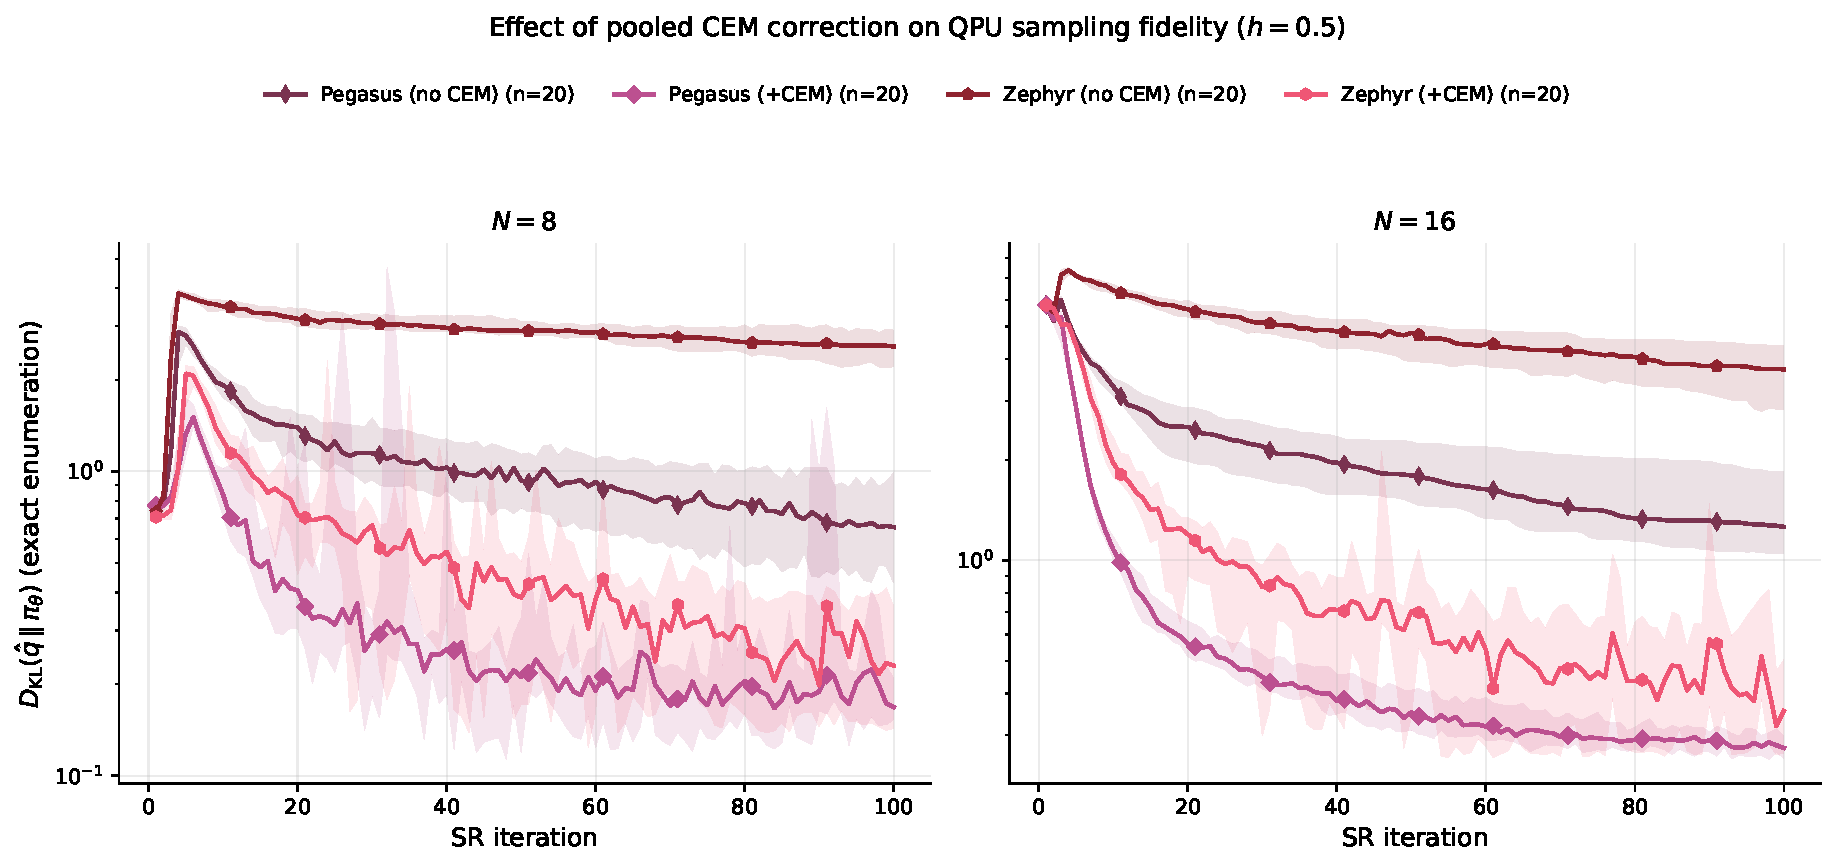
\includegraphics[width=\textwidth]{figures/reanalysis/fig_kl_exact_cem_ablation.pdf}
\caption{Effect of pooled CEM correction on exact $\DKL(\widehat q\Vert\pi_\theta)$, $h=0.5$, $N=8,16$ (median and IQR band, 20 seeds per arm). \texttt{cem=0} (uncorrected) sits nearly an order of magnitude above \texttt{cem=1} throughout training for both devices, with the larger benefit for Zephyr. This is direct evidence that the pooled-CEM estimator of Sec.~\ref{sec:cem-ls} improves the sampled distribution itself, not only the logged training energy.}
\label{fig:kl-cem}
\end{figure*}

Both figures are scoped to $N\le16$ by the same \texttt{KL\_EXACT\_MAX\_N} enumeration limit discussed in Sec.~\ref{sec:validation}; they say nothing directly about $N=64$, where the crossover of Sec.~\ref{sec:limitations} is reported.

\subsection{Consistency between conditional and visible fits}

Figure~\ref{fig:cemvalidation} compares the pooled-CEM estimate $\widehat\beta_{\mathrm{LS}}$ against a direct visible-distribution fit $\widehat\beta_{\mathrm{KL}}=\arg\min_\beta\DKL(\widehat q\Vert\pi_{\theta,\beta})$, obtainable only where $\pi_{\theta,\beta}$ can be enumerated ($N=8,12$). Many points lie near the diagonal, but checkpoint-averaged offsets of order $0.06$–$0.08$ appear, and at least one fit sits at the search boundary $\beta=50$. Agreement is therefore neither uniform nor evidence of exact calibration; it is consistent with -- but does not by itself demonstrate -- the counterexample of Sec.~\ref{sec:cem-limits}, in which the pooled hidden loss can be minimized at the correct $\beta$ even when the visible marginal is substantially wrong.

\begin{figure}[t]
\centering
\panel{.48}{\textbf{(a)}\\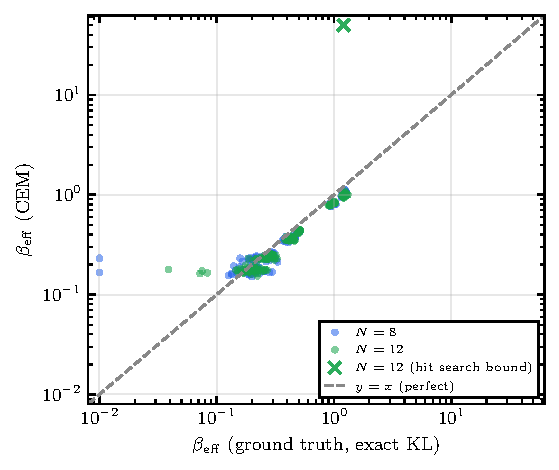
\includegraphics[width=\linewidth]{figures/cem_validation_calibration.pdf}}\hfill
\panel{.48}{\textbf{(b)}\\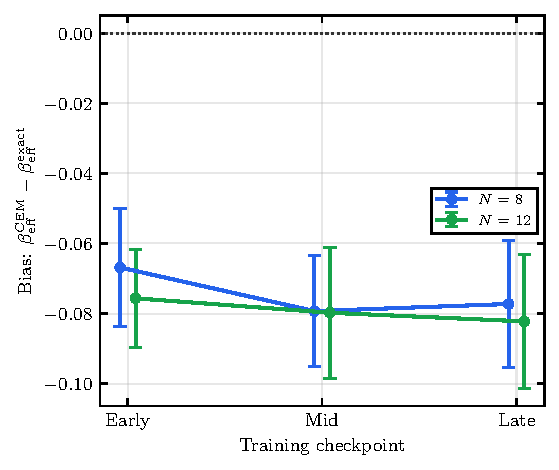
\includegraphics[width=\linewidth]{figures/cem_validation_bias.pdf}}
\caption{(a) Pooled-CEM $\widehat\beta_{\mathrm{LS}}$ against the enumerated visible-fit $\widehat\beta_{\mathrm{KL}}$, $N=8,12$. (b) Checkpoint-averaged offsets. A boundary estimate is annotated and must not be read as a resolved optimum.}
\label{fig:cemvalidation}
\end{figure}

Figure~\ref{fig:cem} illustrates the least-squares fit itself for a representative $N=16$ network: the pooled conditional loss $\mathcal L(\beta)$ has a clear minimum distinguishing $\widehat\beta_{\mathrm{LS}}\approx1.94$ from the candidates $\beta\in\{0.5,1,5\}$.

\begin{figure}[t]
\centering
\panel{.48}{\textbf{(a)}\\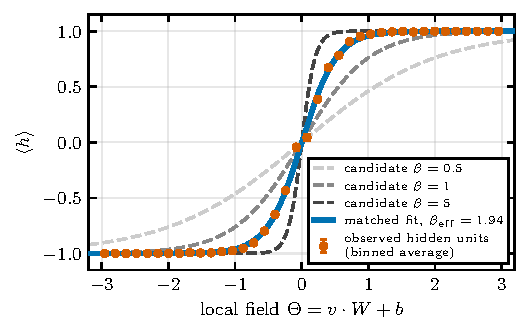
\includegraphics[width=\linewidth]{figures/cem_matching_candidates.pdf}}\hfill
\panel{.48}{\textbf{(b)}\\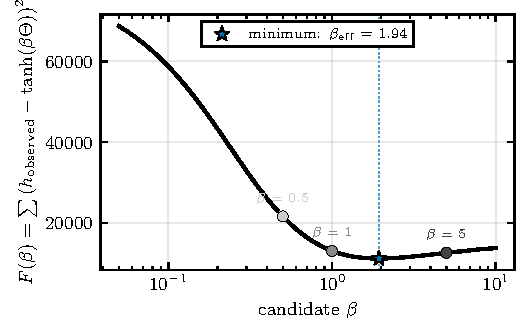
\includegraphics[width=\linewidth]{figures/cem_matching_objective.pdf}}
\caption{Pooled least-squares CEM for a representative $N=16$, $h=1$ network. (a) Binned hidden responses against candidate conditional curves. (b) $\mathcal L(\beta)$, Eq.~\eqref{eq:cem-ls}, minimized near $\beta=1.94$.}
\label{fig:cem}
\end{figure}

\missing{\textbf{Residual reported as a number, not only ``very close.''} Per the evaluation, Fig.~\ref{fig:cemvalidation} and Fig.~\ref{fig:cem} should be accompanied by numerical RMSE, relative error, bias, and boundary-hit frequency across the full $(N,h,\beta_x,\mathrm{seed})$ grid, not a qualitative description. This is a re-tabulation of already-collected fit results and does not require new hardware time, but no script currently outputs these summary statistics (Sec.~\ref{sec:code-gaps}).}


\section{Time-to-accuracy over $N$, $h$, and $\epsilon$}
\label{sec:tta}

\subsection{The existing statistic underestimates retry cost}
\label{sec:tte-issue}

The source report's crossing statistic (Eq.~\eqref{eq:rollingmean}) is converted into a $99\%$-confidence time-to-solution by treating an unsuccessful seed as a full restart at the median successful time:
\begin{equation}
\mathrm{TTE}_{99}=
\begin{cases}
T_r, & p=1,\\[2pt]
T_r\,\dfrac{\ln(0.01)}{\ln(1-p)}, & 0<p<1,
\end{cases}
\label{eq:tte99}
\end{equation}
implemented exactly this way in \texttt{scripts/viz/paper\_figures.py}, function \texttt{tte99\_from\_validated()} (lines 148--174): a failed seed is simply excluded from the set whose median defines $T_r$ and is accounted for only through $p$. This is the standard retry formula for attempts of a \emph{fixed} runtime, but here a successful attempt can stop early at $t^\star$ while an unsuccessful one consumes the full $100$-iteration budget, and $T_r$ is computed only from the (generally shorter) successful attempts -- so the formula omits the cost of the failed full-budget runs it is nominally accounting for. This matters exactly where the reported crossover is claimed: at $N=64$, the reported successful fractions are FPGA $19/20$, Zephyr(+CEM) $19/20$, SA $18/20$, Metropolis $17/20$, Gibbs $16/20$, so between one and four unsuccessful seeds enter the ranking through $p$ alone. Exact binomial 95\% intervals at these counts are wide (e.g.\ $19/20\Rightarrow p\in[0.751,0.999]$), so the sharp distinction the current formula draws between, say, a $20/20$ and a $19/20$ series is not statistically supported by the underlying counts.

\missing{\textbf{Survival-corrected TTE statistic.} None of a fixed-cutoff estimator ($p_\tau=\Pr(T\le\tau)$, $T_{99}(\tau)=\tau\ln(0.01)/\ln(1-p_\tau)$, minimized over a pre-specified grid of $\tau$ with bootstrap CIs), a Kaplan--Meier / right-censored treatment of $t^\star$, or a full retry-process simulation from the empirical distribution of successes and full-budget failures is implemented anywhere in the audited repository (Sec.~\ref{sec:code-gaps}, item T3). Reproducing Fig.~\ref{fig:tte-corrected} [PLACEHOLDER] with one of these three estimators, re-run on the archived per-seed histories (no new device time required), is the single highest-priority numerical fix in this paper.}

\subsection{Criterion dependence: $\epsilon$ and $h$}
\label{sec:eps-h}

The reported crossover uses a single cell: the 1D TFIM at $h=0.5$ with $\epsilon=0.1$ per spin (a total-energy tolerance of $6.4$ at $N=64$). The target distribution changes qualitatively across $h$ -- strongly peaked in the ordered phase, approaching uniform at large field -- so a result at $h=0.5$ is not presumptively representative of the critical or paramagnetic regime. A sweep over $h\in\{0.5,0.7,0.9,1.0,1.1,1.3,1.5\}$ at fixed $N=16$ already exists in code, \texttt{fig\_tte\_vs\_h\_n16()} in \texttt{scripts/viz/paper\_figures.py} (lines 1469--1541), but it is defined and never invoked -- it does not run as part of the current figure-generation pipeline, and it fixes $\epsilon=0.1$ rather than sweeping it. No script anywhere sweeps $\epsilon$ (every figure function hardcodes a single value, $0.1$ for the validated-convergence figures and $0.01$ for the unrelated ITE figures).

\missing{\textbf{Joint $(\epsilon,h)$ time-to-accuracy grid.} Producing Fig.~\ref{fig:tta-grid} [PLACEHOLDER] -- time-to-accuracy curves for $\epsilon\in\{0.1,0.05,0.02,0.01\}$ at $h\in\{0.5,1.0,2.0\}$, or the lower envelope of wall time vs.\ independently evaluated error suggested by the evaluation -- requires: (i) wiring \texttt{fig\_tte\_vs\_h\_n16()} into the run pipeline and generalizing it to also loop over $\epsilon$; (ii) at $N=64$ specifically, re-deriving each crossing from the independent evaluator of Sec.~\ref{sec:validation} rather than the training log, since this is exactly the size and field at which the current crossover claim (Sec.~\ref{sec:limitations}) is made. Only new QPU time is required at cells not already covered by archived checkpoints.}

Figure~\ref{fig:tte-baseline} reproduces the single existing $(\epsilon,h)=(0.1,0.5)$ cell, labelled explicitly as one point in a criterion space rather than as the general result.

\begin{figure}[t]
\centering
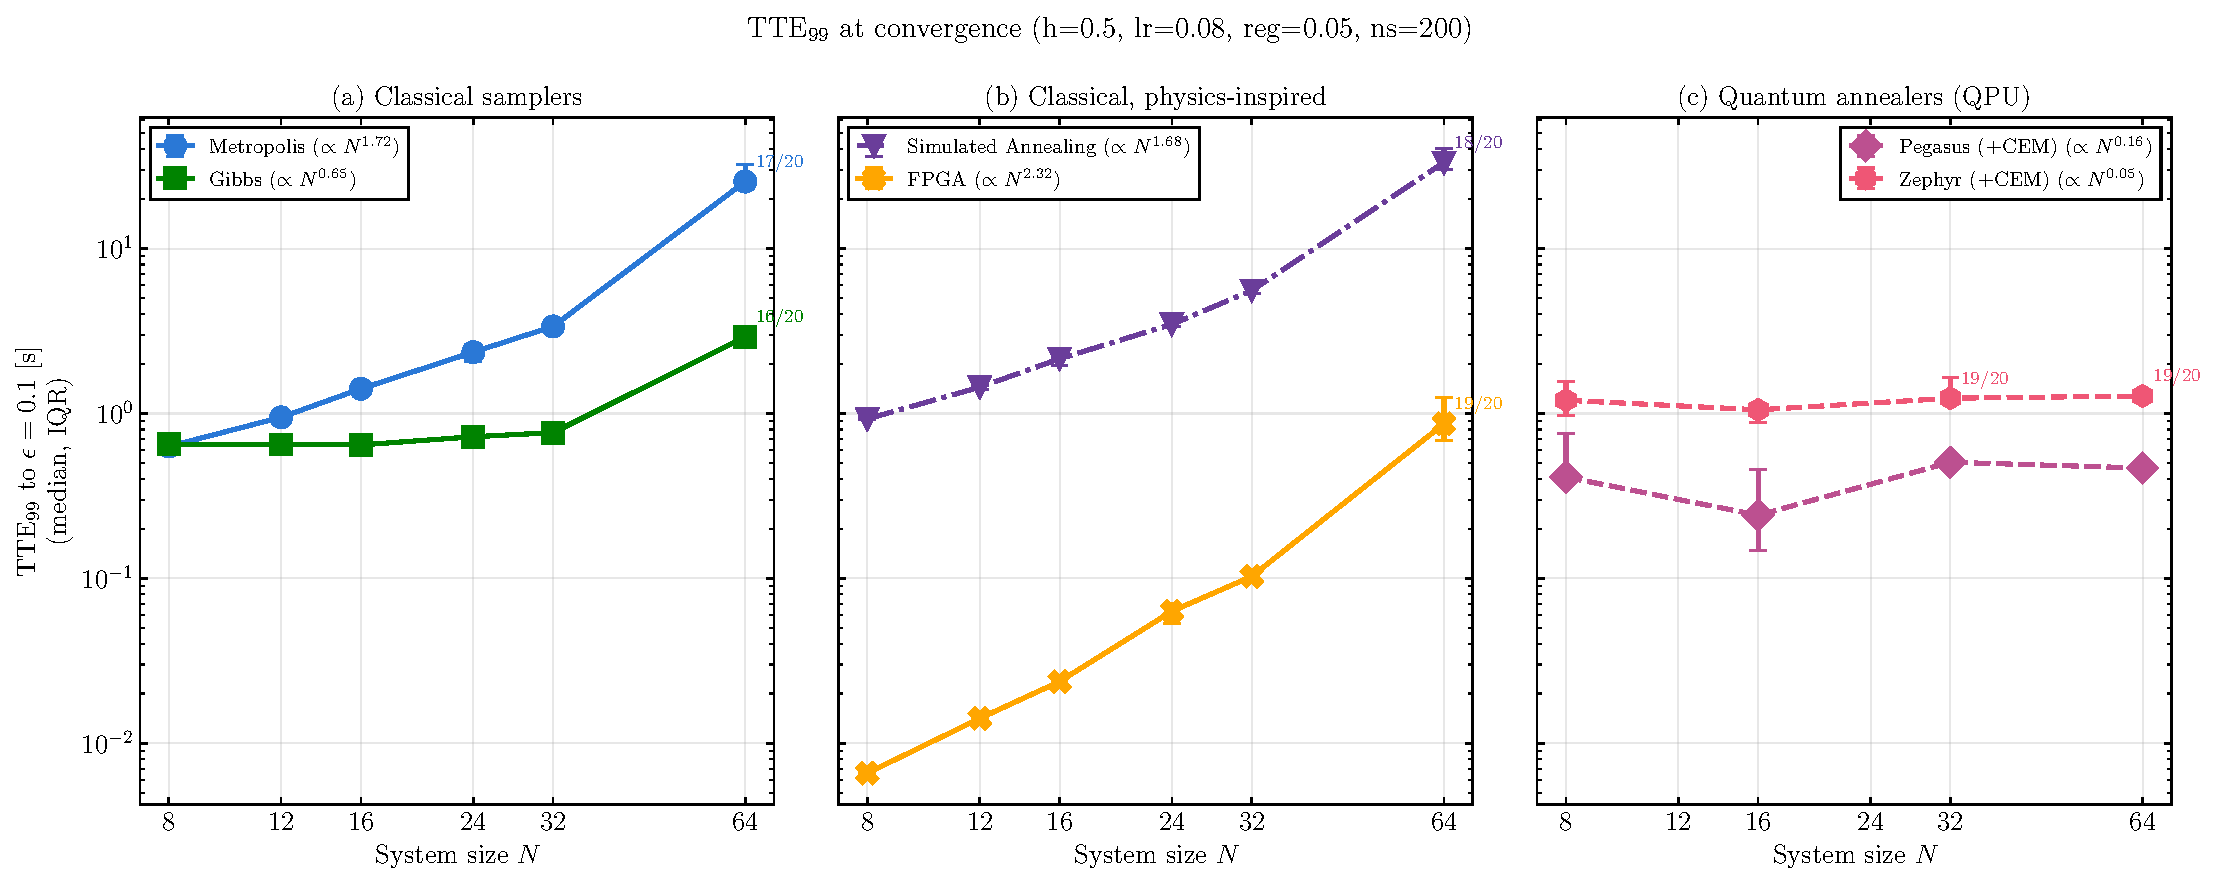
\includegraphics[width=\linewidth]{figures/fig10c_tte99_vs_n_eps0.1.pdf}
\caption{$\mathrm{TTE}_{99}$ (Eq.~\eqref{eq:tte99}) vs.\ $N$ at the single tested cell $h=0.5$, $\epsilon=0.1$. Annotated fractions give the successful-seed count where below $20/20$. This is the only $(\epsilon,h)$ cell for which a full-$N$ curve currently exists; Sec.~\ref{sec:eps-h} explains why it should not be read as representative.}
\label{fig:tte-baseline}
\end{figure}

\subsection{Fixed-protocol vs.\ solver-optimized comparison}

The classical baselines are matched on outer SR settings but not on inner sampling effort: Metropolis restarts with 200 warm-up sweeps plus one sampling sweep, persistent Gibbs uses ten block sweeps after a one-time initialization, and simulated annealing uses 200 warm-up plus 40 cooling sweeps. This fixed-protocol comparison is scientifically useful on its own terms but is not the best-achievable time-to-accuracy of each sampler; sampling-quality figures elsewhere in this project (Fig.~\ref{fig:classical}) show simulated-annealing quality still improving well past 40 sweeps. \missing{\textbf{Solver-optimized comparison.} A second benchmark in which every classical sampler receives the same hyperparameter-tuning budget and independently minimizes its own time-to-accuracy, rather than sharing the outer protocol, is not implemented and is listed as a distinct experiment rather than an edit to the existing one.}

\section{Device time, end-to-end time, and hardware-resource accounting}
\label{sec:resources}

\subsection{Timing boundaries actually measured}

The recorded comparison uses, per backend: D-Wave \texttt{qpu\_access\_time} (programming, anneal, readout), excluding network latency, queueing, and one-time embedding; classical-sampler host-wrapper time after excluding JIT compilation warm-up; and FPGA on-device cycle count divided by its $120\,\mathrm{MHz}$ clock. \texttt{src/encoder.py} (line 557) additionally forms \texttt{total\_sampling\_time\_s = sample\_time\_s + cem\_time}, i.e.\ the device/sampler time plus the host-side CEM computation -- a legitimate device-plus-thermometry-overhead number, but still not host-device transfer, embedding/unembedding construction, chain decoding, or the network round-trip. A separate \texttt{wall\_time\_s} covering an entire run is recorded in some pipelines (\texttt{scripts/hparam/hparam\_optuna.py}, \texttt{scripts/ite/ite\_run.py}, \texttt{scripts/j1j2/j1j2\_convergence\_median.py}) but is not decomposed into the components above and is not the metric plotted in the $\mathrm{TTE}_{99}$ figures.

\missing{\textbf{Two clearly labelled timing series.} (1) device/kernel time, approximately what is already plotted; (2) end-to-end wall time including data preparation, host--device transfer, embedding/unembedding, chain decoding, the CEM computation already tracked in \texttt{total\_sampling\_time\_s}, and network round-trips. A third, practically motivated number -- amortized end-to-end time when an embedding is cached and reused across many training jobs -- is also absent. None of these decompositions exist in the current timing code (Sec.~\ref{sec:code-gaps}, item T5), so Fig.~\ref{fig:e2e-timing} [PLACEHOLDER] requires new instrumentation, not a re-plot.}

Stochastic reconfiguration itself is excluded from the sampler-vs-sampler comparison because it is nominally common across backends; that isolates sampler performance but can hide a regime where the SR solve dominates total training time regardless of sampler speed. We do not currently report total training time alongside the sampler-only comparison; doing so requires no new experiments, only re-aggregating already-logged per-iteration timings.

\subsection{Quantum-annealer hardware-resource accounting}
\label{sec:hw-resources}

The reported near-flat scaling of QPU access time with $N$ (fitted exponents $\propto N^{0.16}$ and $\propto N^{0.05}$ over only four sizes, $N\in\{8,16,32,64\}$) reflects a fixed $20\,\mu\mathrm s$ anneal time and a fixed read count per call; it says nothing by itself about how the physical resources consumed by minor embedding grow with $N$, since a dense $K_{N,N}$ RBM requires longer coupler chains as $N$ grows. \texttt{src/sampler.py} (the D-Wave sampling paths, e.g.\ around line 1478 and 1588) reads only \texttt{info["timing"]["qpu\_access\_time"]} from the returned sample set; grepping the repository for chain-break fraction, physical-qubit count, or embedding-success telemetry (\texttt{chain\_break\_fraction}, \texttt{broken\_chain}, \texttt{num\_qubits}, \texttt{embedding\_success}) returns no hits. The existing embedding-algorithm scripts (\texttt{scripts/exper/embedding\_algo\_comparison.py}, \texttt{parallel\_embedding\_experiment.py}, \texttt{parallel\_embedding\_bench.py}) compare how the choice of embedding algorithm affects training outcome and QPU time, not the qubit-count/chain-length/rescaling telemetry needed here, and no programming/anneal/readout time breakdown is recorded anywhere.

Physical qubit count and chain length, at least, do not require new hardware access: the archived result files log an \texttt{embedding\_info} field (present for $N=8,32,64$, both devices; absent for $N=16$) that already gives exactly this, unused until now. The $N=16$ gap is closeable offline: both devices' live hardware-graph snapshots are cached on disk (\texttt{embeddings/\_hwgraph\_\{Advantage\_system6,Advantage2\_system1\}\_live.json}, the same topology used to generate the other sizes' embeddings), so re-running \texttt{minorminer.busclique} locally against that cached graph -- no QPU or network access -- gives a directly comparable number. Table~\ref{tab:resources} reports the complete series.

\begin{table}[h]
\caption{Physical qubits and chain length for the dense $K_{N,N}$ biclique embedding, both devices. $N=16$ recomputed offline from the cached live hardware-graph snapshot (\texttt{minorminer.busclique}, no QPU access); all other cells read from archived \texttt{embedding\_info}.}
\label{tab:resources}
\begin{ruledtabular}
\begin{tabular}{lrrrrr}
& \multicolumn{2}{c}{Pegasus} & \multicolumn{2}{c}{Zephyr} \\
$N$ & qubits & mean chain & qubits & mean chain \\
\hline
8 & 22 & 1.38 & 16 & 1.00 \\
16 & 64 & 2.00 & 48 & 1.50 \\
32 & 212 & 3.31 & 192 & 3.00 \\
64 & 768 & 6.00 & 956 & 7.47 \\
\end{tabular}
\end{ruledtabular}
\end{table}

Zephyr is cheaper than Pegasus at every size up to $N=32$, then crosses over: at $N=64$ -- the size at which the corrected crossover claim of Sec.~\ref{sec:limitations} is made -- Zephyr requires both more physical qubits (956 vs.\ 768) and longer chains (mean $7.47$ vs.\ $6.00$) than Pegasus, a concrete hardware-resource correlate of Zephyr's consistently worse showing there.

\missing{\textbf{Remaining resource fields.} Chain-break fraction, coefficient-rescaling range, embedding success rate, number of simultaneously available embeddings, and separate programming/anneal/readout time components are still not captured anywhere (Sec.~\ref{sec:code-gaps}, item T5) -- these require reading additional fields from the D-Wave SDK's \texttt{SampleSet.info} that the current code discards, which is only obtainable from a live QPU call, not a re-analysis. A more honest timing model, $t(N)=t_0+aN^p$ with $t_0$ a fixed call overhead, should be fit once these remaining resource series exist; with only four $N$ values any such fit remains descriptive.}

\subsection{FPGA sampler: documentation and fidelity}
\label{sec:fpga}

The FPGA backend (\texttt{FPGASampler} in \texttt{src/sampler.py}, lines 581--892) documents its I/O protocol and configuration (\texttt{num\_rep=1024}, \texttt{num\_steps}, \texttt{num\_sweeps}, \texttt{start\_temp}/\texttt{stop\_temp}, geometric schedule) but not its transition rule or stationary distribution; the update algorithm itself lives in the external, non-vendored \texttt{VeloxQFPGA} Julia package, called from \texttt{scripts/fpga/fpga\_sa\_server.jl} rather than reproduced in this repository. How the 1024 replicas become the $\sim\!200$ samples used by SR \emph{is} documented: lines $\approx$858--865 draw a uniform, without-replacement subsample (\texttt{\_subsample\_rng.choice(..., replace=False)}), with an accompanying comment (on the analogous \texttt{VeloxQStandardSASampler}, lines $\approx$891--909) explaining that uniform subsampling, rather than taking the lowest-energy replicas, is required to avoid biasing $\avg{\Eloc}$. No bitstream, board model, or toolchain version is pinned in code (an optional \texttt{FPGA\_BITSTREAM} environment variable defaults to blank), sample independence across replicas is not tested, and no $\DTV$-style fidelity test analogous to Fig.~\ref{fig:classical} exists for the FPGA (\texttt{scripts/dtv/} contains no FPGA-referencing file).

\missing{\textbf{Complete FPGA algorithmic specification and fidelity test.} (i) the transition/update equations actually implemented in \texttt{VeloxQFPGA}, vendored or cited to a pinned version; (ii) whether the resulting chain has a known stationary distribution and how its effective temperature is controlled; (iii) FPGA model, toolchain, and bitstream version, pinned; (iv) a $\DTV$/$\DKL$ fidelity test at small $N$ analogous to Fig.~\ref{fig:classical}, so the FPGA enters the same non-Gibbs-distortion accounting as the QPU and classical samplers rather than being assessed by energy alone.}

\subsection{Energy accounting}

GPU energy is measured, not modeled: \texttt{src/energy.py}'s \texttt{GPUEnergyMeter} polls \texttt{nvidia-smi --query-gpu=power.draw} on a background thread (default $0.5\,\mathrm s$ interval) and trapezoidally integrates power over explicitly marked active windows that isolate solver/sampling time from SR/CG compute; it does not subtract an idle-power baseline. FPGA energy is not measured at all: \texttt{scripts/viz/plot\_ite.py} (lines 82--86) and \texttt{scripts/viz/paper\_figures.py} (line 1348) both hardcode \texttt{ASSUMED\_POWER\_W\{"fpga/fpga": 45.0\}} and multiply by device time; QPU energy is correctly omitted rather than estimated. The current energy comparison therefore mixes one genuinely measured series (GPU) with one modeled constant (FPGA) and one omission (QPU); \missing{it should either move to supplementary material labelled exploratory, or be rebuilt with measured FPGA board power, idle-baseline subtraction for the GPU meter, and a stated common system boundary for both.}

\section{Limitations and the conditions under which a crossover is observed}
\label{sec:limitations}

\subsection{Correcting the headline claim}
\label{sec:headline}

The source report's abstract and conclusion state that \emph{both} Pegasus and Zephyr overtake FPGA in $\mathrm{TTE}_{99}$ at the largest tested size. The underlying figure does not support this for both devices: at $N=64$, FPGA's $\mathrm{TTE}_{99}$ is $0.87\,\mathrm s$, and the report's own results text calls this ``clearly higher than Pegasus'' -- it does not make the corresponding claim for Zephyr, whose plotted value sits above FPGA's at that size. The defensible statement, and the one this paper adopts, is:

\begin{quote}
Under the device-time metric and the $h=0.5$, $\epsilon=0.1$ convergence criterion, Pegasus(+CEM) has a lower estimated $\mathrm{TTE}_{99}$ than FPGA at $N=64$. Zephyr(+CEM) does not. This is a single observed crossover at one size, one field, and one tolerance, using the training-log crossing statistic of Sec.~\ref{sec:trainingcrossing} and the retry formula whose limitations are discussed in Sec.~\ref{sec:tte-issue} -- not evidence of asymptotic scaling, and not evidence of quantum advantage.
\end{quote}

Every occurrence of the broader ``both QPUs overtake FPGA'' claim in the source material -- abstract, results discussion of Fig.~\ref{fig:tte-baseline}, and conclusion -- should be replaced by this statement or removed.

\subsection{Why the crossover should not yet be generalized}

Three independent limitations, each already established in this paper, bound how far the corrected statement above can be pushed:
\begin{enumerate}
\item \textbf{Validation.} The crossing itself is read from the training log (Sec.~\ref{sec:trainingcrossing}), not from the independent evaluator of Sec.~\ref{sec:validation}; Sec.~\ref{sec:cem-limits} shows explicitly that a stable training-time energy is compatible with a substantially wrong visible distribution.
\item \textbf{Retry accounting.} The $\mathrm{TTE}_{99}$ values being compared understate the cost of unsuccessful seeds (Sec.~\ref{sec:tte-issue}), and the ranking at $N=64$ is decided by exactly the seeds this affects.
\item \textbf{Criterion dependence.} The crossover is reported at one $(\epsilon,h)$ cell out of the space described in Sec.~\ref{sec:eps-h}; whether it persists, disappears, or reverses under a tighter tolerance or a different field is, at present, unknown rather than merely uncertain -- the $\{0.1,0.05,0.02,0.01\}\times\{0.5,1.0,2.0\}$ grid needed to answer this has not been run.
\end{enumerate}
A single number that survives all three checks -- an independently validated, survival-corrected $\mathrm{TTE}_{99}$ crossover confirmed across at least two tolerances and two fields -- does not yet exist. \missing{Table~\ref{tab:crossover} [PLACEHOLDER]: the corrected crossover result, filled in once Secs.~\ref{sec:validation}, \ref{sec:tte-issue}, and \ref{sec:eps-h}'s placeholders are resolved.}

\subsection{Scope excluded from the central claim}

Three further results from the source report are retained only as short, explicitly scoped appendices (App.~\ref{app:sparse}--\ref{app:marshall}) rather than folded into the thermometry-and-validation narrative above, following the evaluation's recommendation: the sparse hardware-native RBM ablation (App.~\ref{app:sparse}), simultaneous embeddings (App.~\ref{app:parallel}), and the Marshall-sign study on frustrated Heisenberg chains (App.~\ref{app:marshall}). None of these three bears on the effective-temperature estimator that is this paper's central contribution, and each has its own, separately scoped limitations recorded in its appendix.

\section{Conclusion}
\label{sec:conclusion}

We isolated, from a broader research-stay report, the single result the evaluation judged most publishable: a partition-function-free, online, pooled conditional-thermometry estimator for quantum-annealer-sampled RBM wavefunctions, formulated here both as the original pooled least-squares fit and as a conditional maximum-likelihood estimator with an explicit score equation (Sec.~\ref{sec:thermometry}). We showed precisely what agreement of hidden conditional means does and does not certify about the sampled visible distribution (Sec.~\ref{sec:cem-limits}), specified the independent, training-blind evaluation protocol needed to certify a reported convergence (Sec.~\ref{sec:validation}), and corrected the report's headline claim to what its own data support: a single, criterion-specific $\mathrm{TTE}_{99}$ crossover of Pegasus, but not Zephyr, over an undocumented FPGA baseline at one system size (Sec.~\ref{sec:headline}).

This draft is intentionally incomplete where the underlying analysis is: every \missinginline{red placeholder} marks a specific figure, table, or theoretical result that the evaluation asked for and that Sec.~\ref{sec:code-gaps} confirms does not yet exist in the implementation repository. None of the required work needs new QPU time except where explicitly noted (the matched small-$N$ QPU sampling-quality run of Sec.~\ref{sec:calibration}, and the $N=64$ cells of the $(\epsilon,h)$ grid in Sec.~\ref{sec:eps-h}); the remainder is re-analysis of already-archived trajectories and new instrumentation of the existing sampling code.

\section*{Data availability}
The implementation and archived report referenced throughout are the repositories audited in Sec.~\ref{sec:code-gaps}; this draft's own source, figures, and bibliography are versioned alongside \texttt{report.tex} in the same project directory. \missinginline{final commit hashes and a DOI to be added once the placeholders above are resolved and the manuscript is frozen for submission.}

\section*{Use of computational assistance}
An AI language model assisted with restructuring this manuscript around the evaluation's recommended framing, deriving the conditional-maximum-likelihood estimator of Sec.~\ref{sec:cem-mle}, and auditing the implementation repository for the code-gap inventory in Sec.~\ref{sec:code-gaps}. It did not run any new experiments; every placeholder in this draft marks work that still needs to be done by the authors.

\appendix

\section{Bias bound for a mismatched sampling distribution}
\label{app:bias}

For any sampler law $q$, the sampled and variational energies (Sec.~\ref{sec:validation}) differ by
\begin{equation}
\widetilde E_q-E_\theta=\sum_v[q(v)-\pi_\theta(v)]\Eloc(v),
\label{eq:bias}
\end{equation}
so that for finite local energies,
\begin{equation}
|\widetilde E_q-E_\theta|\le[\max_v\Eloc(v)-\min_v\Eloc(v)]\,\DTV(q,\pi_\theta).
\label{eq:biasbound}
\end{equation}
A one-spin example saturates this bound and shows it can be numerically large: for $H=-\sigma^x$, $\pi=(0.99,0.01)$, $\psi=\sqrt\pi$, the variational energy is $E_\theta=-2\sqrt{0.99\times0.01}\approx-0.199$, while a sampler with $q=(0,1)$ gives $\widetilde E_q\approx-9.950$ -- far below $E_0=-1$, without contradicting the variational principle, which bounds $E_\theta$, not $\widetilde E_q$. This is why Sec.~\ref{sec:validation} insists on an independently sampled or exactly enumerated $E_\theta$ rather than the training-time $\widetilde E_q$: a small logged $\widetilde E_q-E_0$ does not bound $E_\theta-E_0$ unless $\DTV(q,\pi_\theta)$ is separately controlled.

\section{Repository audit: what code the placeholders in this paper require}
\label{sec:code-gaps}

Table~\ref{tab:codegaps} summarizes an audit of the implementation repository against the eight capabilities this paper's placeholders depend on. ``Present'' means the capability exists and is used in the current pipeline; ``partial'' means related code exists but does not do what is needed; ``absent'' means no such code was found. File paths and line numbers are current as of the audited checkout and should be re-verified against the commit actually used for any figure regenerated from this table.

\begin{table*}[t]
\caption{Code-gap inventory for the placeholders in Secs.~\ref{sec:thermometry}--\ref{sec:resources}. Repository root: \texttt{adiabatic-boltzmann}.}
\label{tab:codegaps}
\begin{ruledtabular}
\begin{tabular}{lp{0.1\textwidth}p{0.55\textwidth}}
Item & Status & Evidence \\
\hline
T1. Conditional-MLE thermometry (Sec.~\ref{sec:cem-mle}) & Absent & \texttt{src/encoder.py:206--219}, \texttt{estimate\_beta\_eff\_cem}, implements only the pooled least-squares objective Eq.~\eqref{eq:cem-ls} via \texttt{scipy.optimize.minimize\_scalar}. No score-equation (Eq.~\eqref{eq:score}) solver exists anywhere in \texttt{src/} or \texttt{scripts/}. \\
T2. Independent frozen-checkpoint evaluator (Sec.~\ref{sec:protocol}) & Partial & \texttt{scripts/exper/exact\_ansatz\_floor.py} performs exact-enumeration \emph{training} (not evaluation of an already-trained, frozen checkpoint with an independent RNG stream); \texttt{scripts/validation/fill\_reference\_energies.py} only caches exact ground-state energies for computing error, not ansatz evaluation. No \texttt{evaluate\_checkpoint}-type script exists; the training-log rolling-mean energy remains the only per-run energy readout used downstream (e.g.\ \texttt{scripts/viz/plot\_ttc.py}). \\
T3. Survival-corrected $\mathrm{TTE}_{99}$ (Sec.~\ref{sec:tte-issue}) & Absent & \texttt{scripts/viz/paper\_figures.py:148--174}, \texttt{tte99\_from\_validated()}, implements exactly Eq.~\eqref{eq:tte99} (median successful time $\times$ retry factor from $p$); no Kaplan--Meier, right-censoring, or fixed-cutoff-$\tau$ formulation is present. \\
T4. Multi-$(\epsilon,h)$ sweep (Sec.~\ref{sec:eps-h}) & Partial & \texttt{fig\_tte\_vs\_h\_n16()} in \texttt{scripts/viz/paper\_figures.py:1469--1541} sweeps $h\in\{0.5,\dots,1.5\}$ at fixed $\epsilon=0.1$, $N=16$, but is defined and never called from the script's entry point. No script sweeps $\epsilon$; every figure function hardcodes one value ($0.1$ or, for unrelated ITE figures, $0.01$). \\
T5. QPU hardware-resource telemetry (Sec.~\ref{sec:hw-resources}) & Absent & The D-Wave sampling paths in \texttt{src/sampler.py} (e.g.\ lines $\approx$1478, $\approx$1588) read only \texttt{info["timing"]["qpu\_access\_time"]}. A repository-wide search for \texttt{chain\_break\_fraction}, \texttt{broken\_chain}, \texttt{num\_qubits}, \texttt{embedding\_success} returns no hits outside third-party packages. \\
T6. End-to-end vs.\ device timing (Sec.~\ref{sec:resources}) & Partial & \texttt{src/encoder.py:557} forms \texttt{total\_sampling\_time\_s = sample\_time\_s + cem\_time} (device time plus thermometry overhead only); \texttt{wall\_time\_s} is recorded in some pipelines (\texttt{scripts/hparam/hparam\_optuna.py}, \texttt{scripts/ite/ite\_run.py}, \texttt{scripts/j1j2/j1j2\_convergence\_median.py}) but is not decomposed into transfer/embedding/decoding/network components. \\
T7. FPGA algorithm documentation and fidelity test (Sec.~\ref{sec:fpga}) & Partial & \texttt{FPGASampler} in \texttt{src/sampler.py:581--892} documents I/O and configuration and, at lines $\approx$858--865/891--909, the uniform-subsampling rule from 1024 replicas to $\sim\!200$ SR samples (with a bias-avoidance rationale in comments). The transition/update rule and stationary distribution are not documented in this repository -- they live in the external, non-vendored \texttt{VeloxQFPGA} Julia package. No bitstream/toolchain version is pinned (\texttt{FPGA\_BITSTREAM} env var, blank by default); no sample-independence test; no $\DTV$-style fidelity test (\texttt{scripts/dtv/} has no FPGA-referencing file). \\
T8. Measured (not modeled) FPGA/GPU energy (Sec.~\ref{sec:resources}) & Partial & GPU energy is genuinely measured: \texttt{src/energy.py}'s \texttt{GPUEnergyMeter} polls \texttt{nvidia-smi --query-gpu=power.draw} and trapezoidally integrates over marked active windows, without idle-baseline subtraction. FPGA energy is a hardcoded constant: \texttt{scripts/viz/plot\_ite.py:82--86} and \texttt{scripts/viz/paper\_figures.py:1348} both set \texttt{ASSUMED\_POWER\_W\{"fpga/fpga": 45.0\}} $\times$ device time. QPU energy is correctly not estimated at all. \\
\end{tabular}
\end{ruledtabular}
\end{table*}

Items T1--T4 are, in order, the estimator this paper is centrally about, the validation step the evaluation called the single most important repair, the statistic underlying the corrected headline claim of Sec.~\ref{sec:headline}, and the sweep needed to know whether that claim generalizes; they should be prioritized in that order. T5--T8 support Sec.~\ref{sec:resources}'s resource accounting and are independent of the thermometry result itself.

\section{Sparse hardware-native RBMs: a resource note}
\label{app:sparse}

At $N=M=16$, $h=1$ ($E_0=-20.4045944748$), exact-expectation training at 3000 iterations improves several sparse masks substantially over 300 iterations (e.g.\ the $0.808594$-removed mask: median error per spin $0.06341\to0.02162$), while the native hardware mask and the sparsest mask change little. At matched (300) iterations, all three classical samplers tested have larger median error than exact expectations on every shared mask. Figure~\ref{fig:sparse} reproduces both comparisons.

\begin{figure}[h]
\centering
\panel{.48}{\textbf{(a)}\\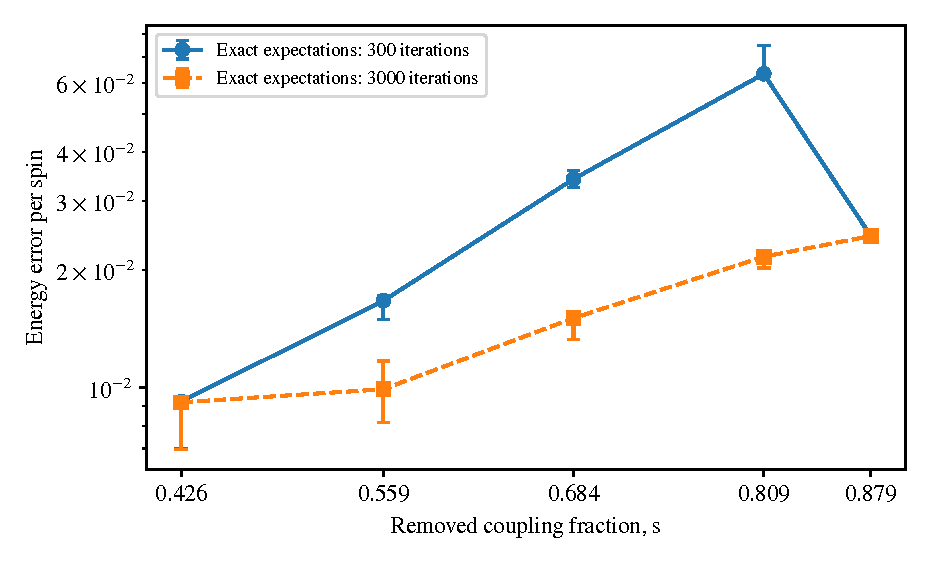
\includegraphics[width=\linewidth]{figures/sparsity_exact_budget.pdf}}\hfill
\panel{.48}{\textbf{(b)}\\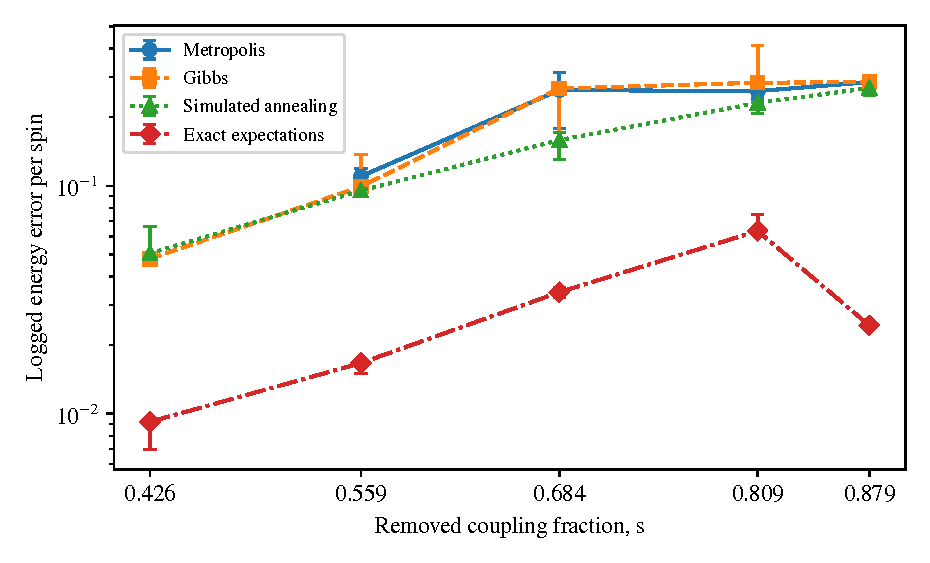
\includegraphics[width=\linewidth]{figures/sparsity_matched_iterations.pdf}}
\caption{(a) Exact-expectation training at 300 vs.\ 3000 iterations across sparsity masks. (b) Matched-iteration (300) comparison of exact expectations against three classical samplers. Five seeds per point; markers are medians, bars span first/third quartiles.}
\label{fig:sparse}
\end{figure}

For any mask $B$, $E_{\mathrm{trained}}\ge E_B^*\ge E_0$, so a favorable exact-expectation result is an achieved upper bound on the best attainable error, not a certified capacity floor -- longer optimization already changes several of these numbers by more than a factor of two. We do not generalize this ablation beyond the tested masks: it shows the tested hardware-derived masks are poor for the tested RBM/TFIM configuration, not that sparse or hardware-native neural quantum states are unsuitable in general.

\section{Simultaneous embeddings: a reliability note}
\label{app:parallel}

Pooling $C$ simultaneously embedded logical copies over $R$ reads returns $CR$ configurations but not necessarily $CR$ independent ones, since shared programming or device fluctuations can correlate copies. In the recorded campaign (one, three, and five copies, three seeds each), four of nine training runs diverge, including two of the three five-copy runs (Fig.~\ref{fig:parallel}). Selecting only converged trajectories would overstate reliability; with three seeds per configuration, this campaign cannot establish a dependable reduction in time-to-validated-state, only that the mechanism is worth a larger study with an explicit per-copy distribution check before pooling.

\begin{figure}[h]
\centering
\panel{.47}{\textbf{(a)}\\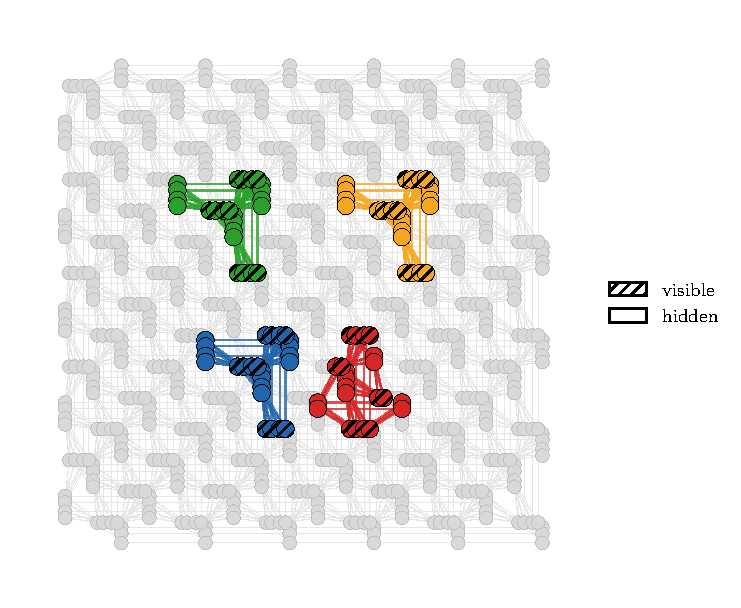
\includegraphics[width=\linewidth]{figures/parallel_embedding/parallel_embedding_np4_pegasus.pdf}}\hfill
\panel{.50}{\textbf{(b)}\\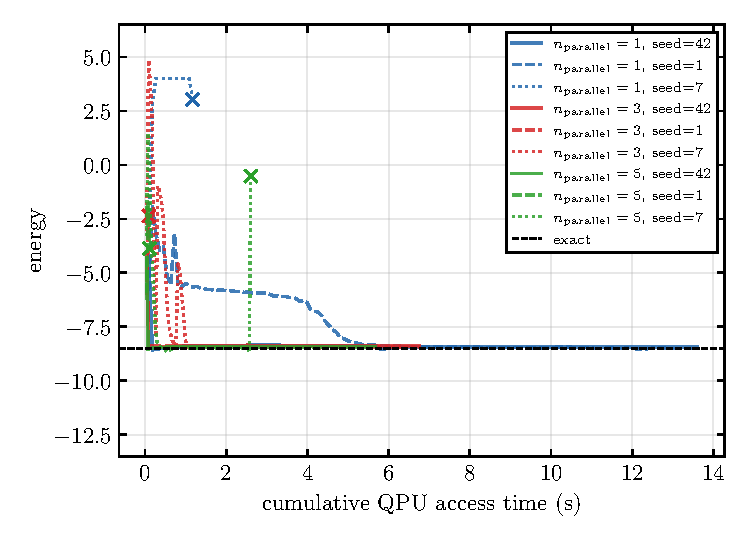
\includegraphics[width=\linewidth]{figures/parallel_embedding/parallel_embedding_np_seeds_qpu_time.pdf}}
\caption{(a) A four-copy Pegasus embedding layout. (b) All nine recorded training trajectories vs.\ cumulative QPU access time; crosses mark divergence.}
\label{fig:parallel}
\end{figure}

\section{Marshall sign rule on the frustrated Heisenberg chain}
\label{app:marshall}

On the $N=8$ antiferromagnetic Heisenberg chain (Metropolis sampling, 200 iterations, three seeds, $J_2/J_1\in[0,1]$), fixing the Marshall sign lowers the energy error by several orders of magnitude at weak frustration, where it supplies the exact off-diagonal sign of every nearest-neighbor exchange, and the improvement shrinks as $J_2$ grows and next-neighbor exchanges (whose sign the transformation does not fix) become significant (Fig.~\ref{fig:marshall}). This is a representational result, not a sampling one: fixing $s(v)$ changes the accessible signed wavefunctions at fixed $|\psi_\theta(v)|^2$, and no improvement in sampler quality removes the restriction once frustration requires signs outside the fixed rule.

\begin{figure}[h]
\centering

\includegraphics[width=.9\linewidth]{figures/marshall_comparison/marshall_comparison_energy.pdf}
\caption{Heisenberg energy error per spin, positive-amplitude vs.\ fixed-Marshall-sign ansatz, $N=8$, three seeds. Bands are recorded standard deviations.}
\label{fig:marshall}
\end{figure}


\clearpage
\bibliography{references}
\end{document}
